\section{Communication Filtering}
The GoT system gives the vehicle's position throughout time. However, since this system use ultrasound waves to register positions in space, it can easily be distorted by interferences and objects on the wave path. It is therefore required to eliminate the big jumps in positions, that could happen in the GoT system, before sending them to the vehicle, see \chapref{Requirements}.

Since the vehicle cannot run faster than \si{3,0\ m \cdot s^{-1}} and that the chosen velocity for the velocity controller is \si{1,4\ m \cdot s^{-1}}, it is possible to define a certain range of positions for a defined time interval. This range is define as a circle, with the a radius as large as the assumed maximum velocity, set to \si{3,0\ m.s^{-1}}, multiplied with the measurement time interval. An example with a \si{1\ s} time interval is given on \figref{GoTFilterSimple}.
\begin{figure}[H]
  \centering
  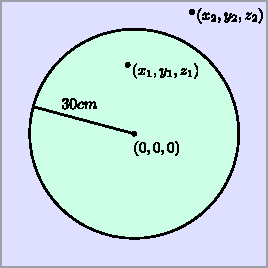
\includegraphics[scale=0.6]{figures/GoTFilterSimple.pdf}
  \caption{Range of possible positions for a maximum speed of \si{3,0\ m \cdot s^{-1}} during a \si{1\ s} interval}
  \label{GoTFilterSimple}
\end{figure}
If the position at a given time, \si{t_0} is \si{(0,0,0)}, the coordinates at the next measurement time, \si{t_1\ =\ t_0\ +\ 1\ s}, should stay within a \si{3,0\ m} radius of the first position.

To ensure the fact that no position jumps is sent to the vehicle, its velocity is measured from the two last sets of coordinates (converted from \si{mm} to \si{m}) and the sampling time of the GoT system (\si{100\ m \cdot s^{-1}}, see \secref{GoTDescription}), see \eqref{eq:velocityGoTCalc}.
\begin{flalign}
\eq{v}{\frac{\sqrt{(X_{2} - X_{{1}})^2 + (Y_{2} - Y_{{1}})^2 + (Z_{2} - Z_{{1}})^2}}{\Delta T}}\unit{m \cdot s^{-1}}
\label{eq:velocityGoTCalc}
\end{flalign}
\hspace{6mm} Where:\\
\begin{tabular}{p{1cm}lll}
  &\si{v}                   & is the velocity of the vehicle                      &\unitWh{m \cdot s^{-1} }\\
  &\si{(X_{2},Y_{2},Z_{2})}   & is the the last set of measured coordinates         &\unitWh{m}\\
  &\si{(X_{1},Y_{1},Z_{1})}   & is the the second last set of measured coordinates  &\unitWh{m}\\
  &\si{\Delta T}            & is the sampling time                                &\unitWh{s}\\
\end{tabular}

Whenever a calculated velocity is greater than the limit of \si{3,0\ m \cdot s^{-1}}, the newest set of coordinates is completely discarded. To calculate the newest velocity afterwards, the previous position, that was not discarded, and the newly measured position are taken, and the sampling time is extended by \si{100\ m \cdot s^{-1}} until a velocity under the limit is measured. When the velocity is under the limit again, the time interval is set to default value again.

However, this type of inconsistency in the system should be fairly rare at a speed of \si{1,4\ m \cdot s^{-1}}, as this so much slower than the limit, which then never will be discarded. And with the GoT is correctly calibrated and the vehicle's environment is clear of interfering obstacles, the distributions will occur rarely and not inflect hard on the system.